\documentclass[twocolumn, letterpaper, 10 pt, conference]{ieeeconf}  % Comment this line out
                                                          % if you need a4paper
%\documentclass[a4paper, 10pt, conference]{ieeeconf}      % Use this line for a4
                                                          % paper

\IEEEoverridecommandlockouts                              % This command is only
                                                          % needed if you want to
                                                          % use the \thanks command


\usepackage[utf8]{inputenc}
\usepackage[T1]{fontenc}
\usepackage{hyperref}
\usepackage{float}
\usepackage{listings}
\usepackage[font=small,labelfont=bf]{caption}
\usepackage{pgfplots, pgfplotstable}
\usepackage{breakcites}
\usepackage{dblfloatfix}
\usepgfplotslibrary{fillbetween}
\pgfplotsset{compat=1.10}
\usepackage{etoolbox}
\usepackage{fixltx2e}

\newtoggle{render_graphs}
\toggletrue{render_graphs}
%\togglefalse{render_graphs}

% Takes six arguments: data table name, x column, y column, error column,
% color and error bar opacity.
% ---
% Creates invisible plots for the upper and lower boundaries of the error,
% and names them. Then uses fill between to fill between the named upper and
% lower error boundaries. All these plots are forgotten so that they are not
% included in the legend. Finally, plots the y column above the error band.
\newcommand{\errorband}[5][]{ % x column, y column, error column, optional argument for setting style of the area plot
\pgfplotstableread[col sep=comma, skip first n=2]{#2}\datatable
    % Lower bound (invisible plot)
    \addplot [draw=none, stack plots=y, forget plot] table [
        x={#3},
        y expr=\thisrow{#4}-2*\thisrow{#5}
    ] {\datatable};

    % Stack twice the error, draw as area plot
    \addplot[draw=none, fill=gray!40, stack plots=y, area legend, #1] table [
        x={#3},
        y expr=4*\thisrow{#5}
    ] {\datatable} \closedcycle;

    % Reset stack using invisible plot
    \addplot [forget plot, stack plots=y,draw=none] table [x={#3}, y expr=-(\thisrow{#4}+2*\thisrow{#5})] {\datatable};
}

\title{Multi-game transfer learning with deep neural networks\\ Independent Project}
\author{
%Stephan Schiffel \\ 
%School of Computer Science / CADIA\\
%Reykjavik University, Iceland\\
%stephans@ru.is \\
%\and
Þorgeir Auðunn Karlsson \\
School of Computer Science \\
Reykjavik University, Iceland\\
thorgeirk11@ru.is\\
}
\date{\today}

\begin{document}
\maketitle
\pagestyle{plain}
\begin{abstract}
    
    Humans have been playing games for centuries and have the ability to learn strategies in one game and apply them to another. This is called transfer learning and has been hard to replicate in general game playing (GGP). GGP agents are capable of independently playing many different games effectively, however they only learn strategies for a single game at a time.
    This paper presents a new approach of transfer learning that can be applied to GGP agents. The approach uses a deep neural network that predicts the likelihood of an action being made in a given state of a game. 
    This model was tested on three different games; Chinese checkers, Connect four and Breakthrough. When pre-trained on different roles for the same game the model achieved higher accuracy after fewer training batches compared to randomly initialized model. This indicates that the approach is an effective way of transfer learning.
    
\end{abstract}  

\section{Introduction}
    General game playing (GGP) seeks to create intelligent agents capable of independently playing many different games effectively without knowing the rules of the game beforehand. Humans have the ability of learning a strategy in one game and apply it on another, effectively transferring the knowledge gained between games. This ability has been hard to replicate in GGP agents.  
    
    GGP competitions have been held for many years and their matches have been recorded. A match consist of series of actions taken from each agent participating in the game. These datasets contain many different games, some of which have over a hundred thousand recorded matches.  Each match was played by a GGP agent, where the agent tried to intelligently pick an optimal action for each state presented. 
    
    Deep neural networks (DNN) have gotten a lot of traction for their ability to learn from massive amounts of raw data and recognize advance patterns \cite{szegedy2015going}. A DNN is composed of series layers, where the input is fed through each layer in turn before arriving at a output layer. In this paper we design a DNN that consists of interchangeable input and output layers for each game and a middle layers that stays persistent between every game. The hypothesis is that this architecture allows the model to learn a game independent representation of a state and can make the training of a unseen game be more effective then otherwise.
    
    %In this paper, the author will employ deep learning techniques and use an ANN to learn the probability of an action being performed on a state for a given game. The deep ANN will have multiple layers and will be designed so that input, output and immediate surrounding layers can be switched out between games. Only the middle part of the hidden layers would remain intact between the games. 
    
    A game state in the game description language (GDL)~\cite{Love2006} consists of propositions that are either true or false and therefore a state can be treated as a boolean array. This boolean array is the input into the ANN. The output of the ANN would be the probability for every action in the game for that given state.
    
    
    
\section{Related work}
    
    General game playing has been studied for over a decade~\cite{Genesereth2005} and many attempts of transfer learning have been made~\cite{banerjee2007general},~\cite{kuhlmann2007graph},~\cite{sato2015transfer} and~\cite{banerjee2006value}. These early works used methods that manipulated the state representation in order to find similar features between games. While effective to some degree they do not use neural networks.
    
    Deep reinforcement learning (RL) has been shown to be capable of playing many different games. Lample and Chaplot showed a RL agent playing DOOM~\cite{lample2016playing}. Stevens and Pradha showed an RL agent playing Tetris~\cite{stevensplaying}. Atari 2600 games have also been played with deep reinforcement learning~\cite{mnih2013playing} and~\cite{mnih2015human}. Deep reinforcement learning has even been shown to master the game GO~\cite{silver2016mastering}.

    However none of these methods have transfer learning between games only between the individual roles of a given game. \cite{hardwick2017evolving} shows a neural evolution technique of applying transfer learning for general game playing.
          
\section{State and action representations}
    The game states are represented in the game description language (GDL)~\cite{Love2006}. GDL is a logic language where the state is represented with facts and terms. By grounding~\cite{schiffel2016grounding} the games description we can find all of the terms that can become true. Since each of these terms are either true or false for any given state they can be represented by a boolean array. 
    
    This boolean array therefore encodes the exact state of the game. E.g. for a very simple game like Tic Tac Toe the state would be represented with a boolean array of length $9*9*9+2$. That is, there are 9 cells and each of them can be an x, an o or empty and alternating the control between the two different roles is also needed. 
    
    The input into the neural network is a normalized version of this array, where true and false are represented by $1$ and $-1$ respectively.

    The actions are represented as a one hot encoding and the number of actions depend on the game and the role of a game. However the number of actions is not dependent on the state it self, that is the neural network doesn't know which actions are legal given a state and therefore doesn't limit the number of actions. The actions are also not always the same between all the roles of a game, so the one hot encoding of the actions can be different between the roles of a given game.

\section{Selected Games}
    Three games were chosen based on the amount of available data and authors familiarity with them; Connect four, six player Chinese checkers and Breakthrough. The data behind each game is divided between the different roles of the game, both Connect four and Breakthrough have two roles, while Chinese checkers has six roles. All of the games are turn based and at each step of the game only a single role takes an action. 
     
    \subsection{Chinese checkers}
    Chinese checkers is a strategy board game where up to six players compete on a star shaped board. This game has the largest state representation of the three games tested and when turned into a boolean array it is of size 253. The actions performed in this game depend on the role, that is the actions are not shared between the roles and one role cannot perform some of the actions of another role. Each role has at most 90 actions that it can perform.
    
    \begin{figure}[H]
        \centering
        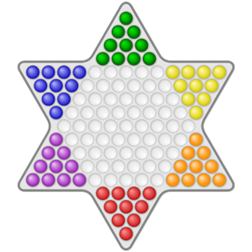
\includegraphics[scale=0.8]{Images/chinese_checkers.png}
        \caption{Chinese checkers has a star shaped board with 6 players.}
        \label{fig:single_role_model}
    \end{figure}
    
    \subsection{Connect four}
    Connect four is a two player puzzle game. This game is the simplest of the three games tested with a state representation of size 127 and only at most 8 actions. The actions are shared between the roles, that is each action is the same for each role. 
    
    \begin{figure}[H]
        \centering
        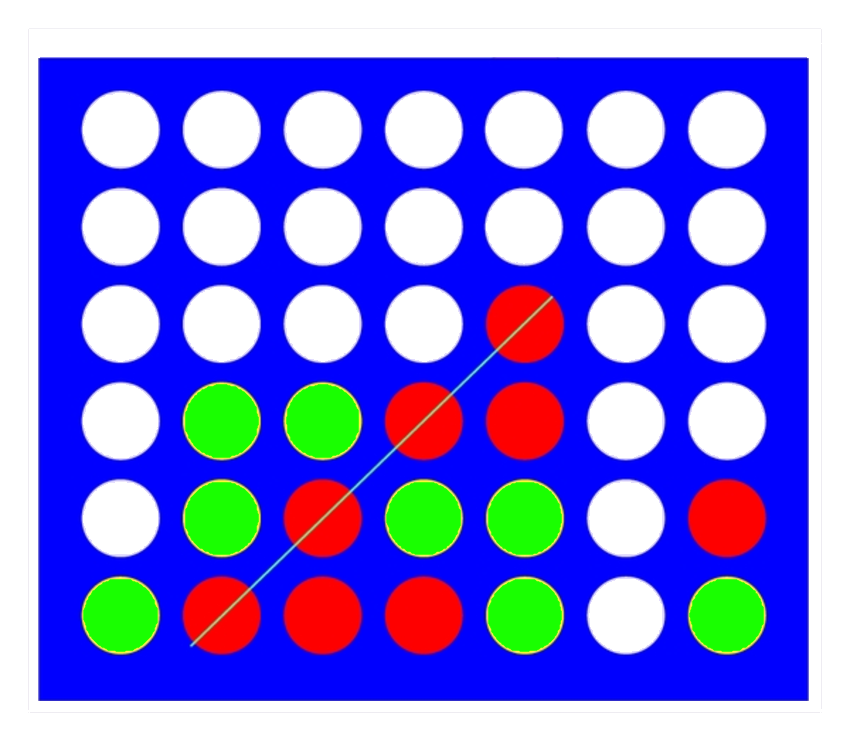
\includegraphics[scale=0.7]{Images/connect4.png}
        \caption{Connect four. This shows a winning state for red on a diagonal line.}
        \label{fig:single_role_model}
    \end{figure}
    
    \subsection{Breakthrough}
    Breakthrough is a two player strategy board game. This game has a state representation of size 130 and has 155 actions. The actions are not shared between the roles, same as in Chinese checkers. 

    \begin{figure}[H]
        \centering
        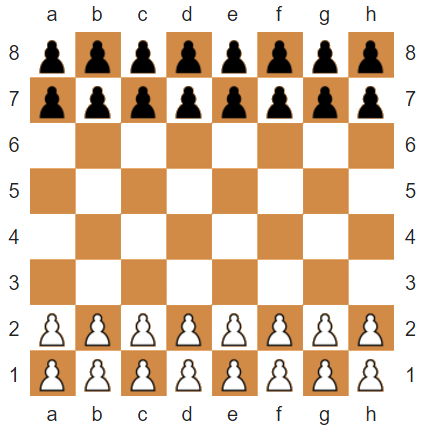
\includegraphics[scale=0.8]{Images/breakthrough.png}
        \caption{Breakthrough board has the same shape as a chess board, the difference is that there are only pawns.}
        \label{fig:single_role_model}
    \end{figure}

%\section{Things to keep in mind}
%    \begin{itemize}
%        \item Imperfect data. \\
%            Always keep in mind that the data is not perfect and often agents perform poorly. This will affect your model and make it harder for it to achieve high accuracy. 

%        \item Amount of data.\\
%            The amount of data is always a factor to consider when training a classifier. Connect four, Breakthrough and Chinese checkers were selected because they contain the most data. The amount of data is however not great, for example Chinese's checkers for role0 there are 5892 entries, which is not a lot.

%       \item Split up the roles. \\ 
%            That is do not train the model on both roles without separation, since the strategy for each role is different and the network could get confused.
%    \end{itemize}
    

\section{Design of the models}
    Deep neural networks (DNN) are structured in a hierarchical fashion. Input into a network is fed through a series of layers before an output layer is reached. Studies have shown that it's representation of the data increases in complexity at each layer of the network. E.g. the lowest layers in the Inception model~\cite{szegedy2015going}, recognize only basic lines and moving up the hierarchy, the layers recognize increasingly complex shapes and patterns.
    
    All of the models are designed with the assumption that a DNN learns in this hierarchical fashion. That is, lower layers learn low level representations and higher level layers increase the complexity of the representation. Therefore all of our models are split into three components:
    \begin{itemize}
        \item The first few layer learn how to read the input state into some abstract representation and 
        \item the next few layers learn how to extract important features out of this abstract representation and 
        \item finally the last layers decide on which action is best, given those features.
    \end{itemize}
    
    The models consists of these three components; input, output and middle. Both the input and output components are changed out for each game since they handle game specific mapping and targeting. However the middle component stays persistent between every game, since it is responsible of learning the abstract reasoning and game independent representation of a state.

    In this paper we created three different models with increasing complexity to achieve different learning goals. All of the models are created with Keras~\cite{chollet2015keras}. The models are single role, multi-role and multi-game. All of these models have the same foundation and will be described in more detail below.

    \subsection{Network structure}
        The network is build up of these three components. 
        
        \subsubsection{Input component} contains a fully connected layer with 200 nodes, however the input size depends on the game since their representation is of varying sizes.
    
        \subsubsection{Output component} contains two fully connected layers and their sizes depend on the game. For both Chinese checkers and Breakthrough the first layer is of size 200, while for Connect four it is of size 50. The last layer has a size equal to the number of actions for a given role.
        
        \subsubsection{Middle component} contains two 500 node fully connected layers with a 50\% dropout~\cite{hinton2012improving} between them.

        All of the layers use a rectified linear activation (Relu)~\cite{nair2010rectified} except the last layer in the output component. It has a softmax activation which is used to determine the probability of each action.
        
    \subsection{Models}
        \subsubsection{Single role} The simplest model only learns from a single role in one particular game. As can be seen from figure-\ref{fig:single_role_model}, this model connects the three components with out any branching.

        \subsubsection{Multi-role} This model has a single input component and multiple output components. This is due to the fact that an input conponent depends only on the game while the output conponents are role dependent. To see how the model was created see the code in figure-\ref{fig:multi_role_model_code} and the model visualization in figure-\ref{fig:multi_role_model}.

        \subsubsection{Multi-game} The multi game model consists of many input and output components where the middle layer is shared between all of the components. See the model visualization in figure-\ref{fig:multi_role_model} 

    \subsection{Fully connected layers}
        Since all games written in the GDL language,~\cite{Love2006}, are Markov decision problems~\cite{thie1983markov}, the history for a given state has no effect on the decision made in that state. The author decided not to invest time in recurrent neural networks (RNN)~\cite{medsker2001recurrent}, for this problem. However it would be interesting to see if training an RNN would improve the accuracy since it could learn the play style of each agent.

    
    \subsection{Measure of accuracy}
        The output of each model is a vector representing the likelihood of an action being performed for the current input state. All of the models use a soft-max classifier to achieve this probability vector. Mean squared error (MSE) was used to measure the effectiveness as it has been shown to be an effective loss function~\cite{silver2016mastering}. This loss function is used to measure how far the prediction is from the actual label.
        
        There are two ways to measure accuracy for this problem. The first is to use the loss function, as it gives an estimate of how far off the prediction is. The second is to use the frequency of the network predicted the correct label. The only problem with the second approach is that if for example two actions are equally likely on a given state then the network will only achieve 50\% accuracy on that state.
        
        For this paper the second approach was used to measure accuracy, that is, how often the model predicted the correct label for a given state.
    
\section{Experimental setup}
    There were three experiment types conducted; single role, multi-role and multi-game experiments. All of the  experiments were run over a 100 times and a 95\% confidence interval is shown on the results.
    
    All of the experiments were done on all three games where the batch consits of 128 samples. The experiments were run for 15.000 batches and after each training batch the model was estimated on unseen validation data and the accuracy plotted.  
    
    \subsection{Single Role Experiments}
        The single role experiment is trained on a randomly initialized model for 50.000 batches. This was done to show how the learning curves evolved for each of the games. It also serves as a baseline for the other experiments and are used to compare the performance of the other approaches. 
    
    \subsection{Multiple Role Experiments}
        The multi-role experiments first train on the same game using all other roles except the first one and then train on the first role. The learning curve for this pre-trained model is compared to a randomly initialized model. This experiments should give an indication of the effectiveness of the middle layer to understand a single game.
    
    \subsection{Multiple Game Experiments}
        The multi-game experiments first training on the other two games before training on the test game. The learning curve of this pre-trained model is also compared to a randomly initialized model. Note that the number of games that are used to pre-train the model is only two. The experiments should likewise give a indication of the effectiveness of the middle layer to handle multiple games. 

%%%%%%%%%%%%%%%%%%%%%%%%%%%%%%%%%%%%%%%%
%%%%%%%%%%%%%%%%%%%%%%%%%%%%%%%%%%%%%%%%
%\iffalse
%%%%%%%%%%%%%%%%%%%%%%%%%%%%%%%%%%%%%%%%
%%%%%%%%%%%%%%%%%%%%%%%%%%%%%%%%%%%%%%%%

\section{Results}
This section details the results from all three types of experiments. All of the following graphs have the same structure, the y axis is the accuracy achieved and the x axis is the number of training batches trained. The lines indicate the mean accuracy where the red squares and the blue circles indicates the pre-trained and randomly initialized models, respectively. The area around each line indicates the 95\% confidence intervals.

\subsection{Single-role experiment}
The single-role experiment, see figure-\ref{fig:single-role}, shows the learning curves for the individual games. Connect four, Breakthrough and Chinese checkers are represented by the red squares, blue circles and green diamonds, respectively. The graph shows that the accuracy for each game is different, which is mainly due to the complexity of the games. This experiment serves as a baseline for all of the games and was run for 50.000 batches.

\begin{figure}[H]
    \begin{tikzpicture}
        \begin{axis}[
            ymin= 0,
            xlabel=Batches Trained,
            ylabel=Accuracy on validation set,
            legend pos= south east,
            legend cell align=left,
            yticklabel={\pgfmathparse{\tick*100}\pgfmathprintnumber{\pgfmathresult}\%}
        ]
            \errorband[red, opacity=0.5,forget plot]{data/connect4_long_run.csv}{0}{1}{2}
            \addplot
                +[thick, mark=square*, mark options={fill=red}, mark repeat=5, mark size=2, red!50!black] 
                table [x index=0, y index=1,col sep=comma]
                {data/connect4_long_run.csv};

            \errorband[blue, opacity=0.5,forget plot] {data/breakthrough_long_run.csv}{0}{1}{2}
            \addplot
                +[thick, mark=*, mark options={fill=blue}, mark repeat=5, mark size=2, blue!50!black] 
                table [x index=0, y index=1,col sep=comma]
                {data/breakthrough_long_run.csv};

            \errorband[green, opacity=0.5,forget plot]{data/chinese_checkers_6_long_run.csv}{0}{1}{2}
            \addplot
                +[thick, mark=diamond*, mark options={fill=green}, mark repeat=5, mark size=2.5, green!50!black] 
                table [x index=0, y index=1,col sep=comma]
                {data/chinese_checkers_6_long_run.csv};

            \legend{Connect four, Breakthrough, Chinese Checkers}
        \end{axis}
        \node[align=center,font=\bfseries, xshift=2em, yshift=1em] (title) 
            at (current bounding box.north)
            {Single-role run for 50.000 batches};
    \end{tikzpicture}
    \caption{Here is the baseline runs for all of the games when run for 50.000 batches. All of these runs were done on a randomly initialized models. The area around each line represents the 95\% confidence interval.}
    \label{fig:single-role}
\end{figure}

\subsection{Multi-role, Connect four}
As can be seen in figure-\ref{fig:connect4}, the pre-trained model has an advantage early on and achieves much higher accuracy for the first thousand batches. However the graph also indicates that the gap between the two models shrinks substantially as the learned batch number increases.  

\begin{figure}[H]
    \begin{tikzpicture}
        \begin{axis}[
            ymin= 0,
            xlabel=Batches Trained,
            ylabel=Accuracy on validation set,
            legend pos= south east,
            legend cell align=left,
            yticklabel={\pgfmathparse{\tick*100}\pgfmathprintnumber{\pgfmathresult}\%}
        ]
            \errorband[red, opacity=0.5,forget plot]{data/connect4_pretrained_15000.csv}{0}{1}{2}
            \addplot
                +[thick, mark=square*, mark options={fill=red}, mark repeat=20, mark size=2, red!50!black] 
                table [x index=0, y index=1,col sep=comma]
                {data/connect4_pretrained_15000.csv};
                   
            \errorband[blue, opacity=0.5,forget plot] {data/connect4_15000.csv}{0}{1}{2}
            \addplot
                +[thick, mark=*, mark options={fill=blue}, mark repeat=20, mark size=2, blue!50!black] 
                table [x index=0, y index=1,col sep=comma]
                {data/connect4_15000.csv};
            
            \legend{Pre-trained, Random Init}
        \end{axis}
        \node[align=center,font=\bfseries, xshift=2em, yshift=1em] (title) 
            at (current bounding box.north)
            {Connect four};
    \end{tikzpicture}
    \caption{Connect four pre-trained vs randomly initialized. 
        The lines indicate mean accuracy where the red squares and blue circles represent the pre-trained and randomly initialized models, respectively. The areas around the lines are the 95\% confidence intervals.
    }
    \label{fig:connect4}
\end{figure}

\subsection{Multi-role, Breakthrough}
For the Breakthrough test, see figure-\ref{plot:breakthrough}, we can also clearly see that the pre-trained model has an advantage early on and achieves much higher accuracy for the first thousand batches. Note that the standard deviation is much larger then for Connect four, which should be expected since this game is more complex. The standard deviation is also lower on the pre-trained model which also is a good indicator that the training has learn some weights that are in general better suited for training. 

The gap between the pre-trained and random models dose not shrink all too much for the first 3000 batches. However these results should be taken with a grain of salt since the accuracy of both models is very poor, less than 30\%.

\begin{figure}[H]
    \begin{tikzpicture}
        \begin{axis}[
            ymin= 0,
            xlabel=Batches Trained,
            ylabel=Accuracy on validation set,
            legend pos= south east,
            legend cell align=left,
            yticklabel={\pgfmathparse{\tick*100}\pgfmathprintnumber{\pgfmathresult}\%}
        ]
            \errorband[red, opacity=0.5, forget plot]{data/breakthrough_pretrained_15000.csv}{0}{1}{2}
            \addplot
                +[thick, mark=square*, mark options={fill=red}, mark repeat=20, mark size=2, red!50!black] 
                table [x index=0, y index=1,col sep=comma]
                {data/breakthrough_pretrained_15000.csv};
               
            \errorband[blue, opacity=0.5,forget plot]{data/breakthrough_15000.csv}{0}{1}{2}
            \addplot
                +[thick, mark=*, mark options={fill=blue}, mark repeat=20, mark size=2, blue!50!black] 
                table [x index=0, y index=1,col sep=comma]
                {data/breakthrough_15000.csv};
            
               
            \legend{Pre-trained, Random Init}
        \end{axis}
        \node[align=center,font=\bfseries, xshift=2em, yshift=1em] (title) 
            at (current bounding box.north)
            {Breakthrough};
    \end{tikzpicture}
    \caption{Breakthrough. The lines indicate mean accuracy where the red squares and blue circles represent the pre-trained and randomly initialized models, respectively. The areas around the lines are the 95\% confidence intervals.}
    \label{plot:breakthrough}
\end{figure}

\subsubsection{Multi-role, Chinese checkers}
For the Chinese checkers experiment, see figure-\ref{fig:cc6}. %This game was the most complex game of the three and as can be seen the pre-training, although achieving on average better results has so wild fluctuations that is not guaranteed to out perform a randomly initialized model. 

Note that in contrast to Breakthrough the pre-trained model has a higher standard deviation than the random initialized model.

\begin{figure}[H]
    \begin{tikzpicture}
        \begin{axis}[
            ymin= 0,
            xlabel=Batches Trained,
            ylabel=Accuracy on validation set,
            legend pos= south east,
            legend cell align=left,
            yticklabel={\pgfmathparse{\tick*100}\pgfmathprintnumber{\pgfmathresult}\%}
        ]
            \errorband[red, opacity=0.5,forget plot]{data/chinese_checkers_6_pretrained_interval_data.csv}{0}{1}{2}
            \addplot
                +[thick, mark=square*, mark options={fill=red}, mark repeat=20, mark size=2, red!50!black] 
                table [x index=0, y index=1,col sep=comma]
                {data/chinese_checkers_6_pretrained_interval_data.csv};
                
            \errorband[blue, opacity=0.5,forget plot]{data/chinese_checkers_6_interval_data.csv}{0}{1}{2}
            \addplot
                +[thick,mark=*, mark options={fill=blue}, mark repeat=20, mark size=2, blue!50!black] 
                table [x index=0, y index=1,col sep=comma]
                {data/chinese_checkers_6_interval_data.csv};
            
            
            \legend{Pre-trained, Random Init}
        \end{axis}
        \node[align=center,font=\bfseries, xshift=2em, yshift=1em] (title) 
            at (current bounding box.north)
            {Chinese Checkers};
    \end{tikzpicture}
    \caption{Chinese checkers. The lines indicate mean accuracy where the red squares and blue circles represent the pre-trained and randomly initialized models, respectively. The areas around the lines are the 95\% confidence interval.  }
    \label{fig:cc6}
\end{figure}


\section{Multi-game experiments}
Here are the results from the mulit-game experiments. 
\begin{figure}[H]
    \begin{tikzpicture}
        \begin{axis}[
            ymin= 0,
            xlabel=Batches Trained,
            ylabel=Accuracy on validation set,
            legend pos= south east,
            legend cell align=left,
            yticklabel={\pgfmathparse{\tick*100}\pgfmathprintnumber{\pgfmathresult}\%}
        ]
            \errorband[green, opacity=0.5,forget plot]{data/bt_trained_on_cc6+con4_(100trials).csv}{0}{1}{2}
            \addplot
                +[thick,mark=diamond*, mark options={fill=green}, mark repeat=20, mark size=3, green!50!black] 
                table [x index=0, y index=1,col sep=comma]
                {data/bt_trained_on_cc6+con4_(100trials).csv};
               
            \errorband[blue, opacity=0.5,forget plot]{data/breakthrough_interval_data.csv}{0}{1}{2}
            \addplot
                +[thick,mark=*, mark options={fill=blue}, mark repeat=20, mark size=2, blue!50!black] 
                table [x index=0, y index=1,col sep=comma]
                {data/breakthrough_interval_data.csv};
            
            
            \legend{Trained on CC6 and Con4, Random Init}
        \end{axis}
        \node[align=center,font=\bfseries, xshift=2em, yshift=1em] (title) 
            at (current bounding box.north)
            {Breakthrough};
    \end{tikzpicture}
    \caption{Multi-game trained model (green diamonds) vs randomly initialized model (blue circles). The pre-trained model is trained on Chinese checkers 6 (CC6) and Connect four (Con4).  The area around each line represents the 95\% confidence interval.  }
    \label{fig:cc6}
\end{figure}

\begin{figure}[H]
    \begin{tikzpicture}
        \begin{axis}[
            ymin= 0,
            xlabel=Batches Trained,
            ylabel=Accuracy on validation set,
            legend pos= south east,
            legend cell align=left,
            yticklabel={\pgfmathparse{\tick*100}\pgfmathprintnumber{\pgfmathresult}\%}
        ]
            \errorband[green, opacity=0.5,forget plot]{data/cc6_trained_on_bt+con4_(100trials).csv}{0}{1}{2}
            \addplot
                +[thick,mark=diamond*, mark options={fill=green}, mark repeat=20, mark size=3, green!50!black] 
                table [x index=0, y index=1,col sep=comma]
                {data/cc6_trained_on_bt+con4_(100trials).csv};
               
            \errorband[blue, opacity=0.5,forget plot]{data/chinese_checkers_6_interval_data.csv}{0}{1}{2}
            \addplot
                +[thick,mark=*, mark options={fill=blue}, mark repeat=20, mark size=2, blue!50!black] 
                table [x index=0, y index=1,col sep=comma]
                {data/chinese_checkers_6_interval_data.csv};
            
            \legend{Trained on BT and Con4, Random Init}
        \end{axis}
        \node[align=center,font=\bfseries, xshift=2em, yshift=1em] (title) 
            at (current bounding box.north)
            {Chinese Checkers};
    \end{tikzpicture}
    \caption{ Multi-game trained model (green diamonds) vs randomly initialized model (blue circles). The pre-trained model is trained on Breakthrough (BT) and Connect four (Con4).  The area around each line represents the 95\% confidence interval. }
    \label{fig:cc6}
\end{figure}


\begin{figure}[H]
    \begin{tikzpicture}
        \begin{axis}[
            ymin= 0,
            xlabel=Batches Trained,
            ylabel=Accuracy on validation set,
            legend pos= south east,
            legend cell align=left,
            yticklabel={\pgfmathparse{\tick*100}\pgfmathprintnumber{\pgfmathresult}\%}
        ]
            \errorband[green, opacity=0.5,forget plot]{data/con4_trained_on_cc6+bt_(240trials).csv}{0}{1}{2}
            \addplot
                +[thick,mark=diamond*, mark options={fill=green}, mark repeat=20, mark size=3, green!50!black] 
                table [x index=0, y index=1,col sep=comma]
                {data/con4_trained_on_cc6+bt_(240trials).csv};
               
            \errorband[blue, opacity=0.5,forget plot] {data/connect4_interval_data.csv}{0}{1}{2}
            \addplot
                +[thick, mark=*, mark options={fill=blue}, mark repeat=20, mark size=2, blue!50!black] 
                table [x index=0, y index=1,col sep=comma]
                {data/connect4_interval_data.csv};
            
            \legend{Trained on BT and CC6, Random Init}
        
        \end{axis}
        \node[align=center,font=\bfseries, xshift=2em, yshift=1em] (title) 
            at (current bounding box.north)
            {Connect four};
    \end{tikzpicture}
    \caption{ Multi-game trained model (green diamonds) vs randomly initialized model (blue circles). The pre-trained model is trained on Breakthrough (BT) and Chinese checkers (CC6).  The area around each line represents the 95\% confidence interval. }
    \label{fig:connect4}
\end{figure}

\section{Future Development}

\color{red}
    Missing
\color{black}

    \subsection{Ideas for further development}
    \begin{itemize}
        \item Train with RNN.\\
            Split the data by the step counter for each match and train it on a RNN. This could learn a play strategy for each role.
        \item Shuffle the state and action representations.\\
            To reuse the same data we could shuffle the bit array and train the model on many different state and action representations for a single game. This could force the network to learn the lower and higher representation of the game in the appropriate layers and move the logic reasoning to the middle layer. 
        \item Training with frozen middle layer. \\
            Training on multiple roles and then freezing the middle layer results in better performance when training on a unseen role.
        \item Neural evolution.\\
            Introduce smarter middle layer with neural evolutionary approch.
    \end{itemize}
    
  

\section{Conclusions}
\color{red}
    Missing
\color{black}


%%%%%%%%%%%%%%%%%%%%%%%%%%%%%%%%%%%%%%%%
%%%%%%%%%%%%%%%%%%%%%%%%%%%%%%%%%%%%%%%%
%\fi
%%%%%%%%%%%%%%%%%%%%%%%%%%%%%%%%%%%%%%%%
%%%%%%%%%%%%%%%%%%%%%%%%%%%%%%%%%%%%%%%%

\bibliographystyle{IEEEtran}
\bibliography{refs.bib}

\newpage
\appendix


\begin{figure}[H]
    \centering
    \caption{Single role model. Network created with keras and is the simplest model with only a single input and output and is intended to only train on a single role for a given game. Image generated by Tensorboard. }
    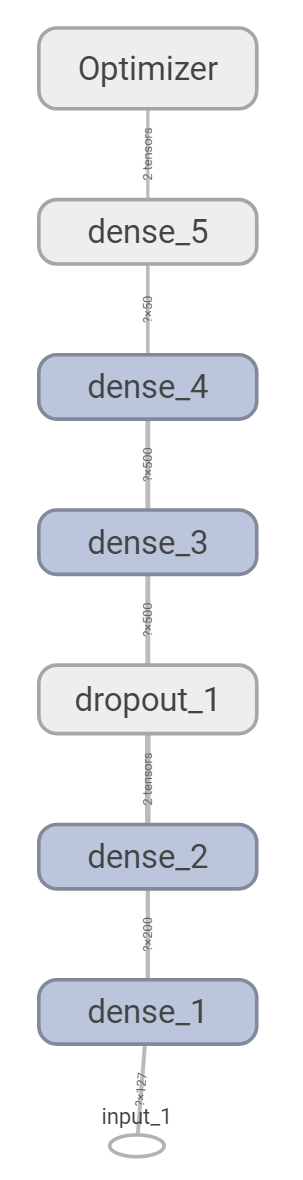
\includegraphics[scale=0.5]{Images/single_role_keras.png}
    \label{fig:single_role_model}
\end{figure}

\begin{figure}[H]
    \centering
    \caption{Multi-role model. This network is created with Kears and has a single input but multiple outputs, one for each role. Image generated by Tensorboard. }
    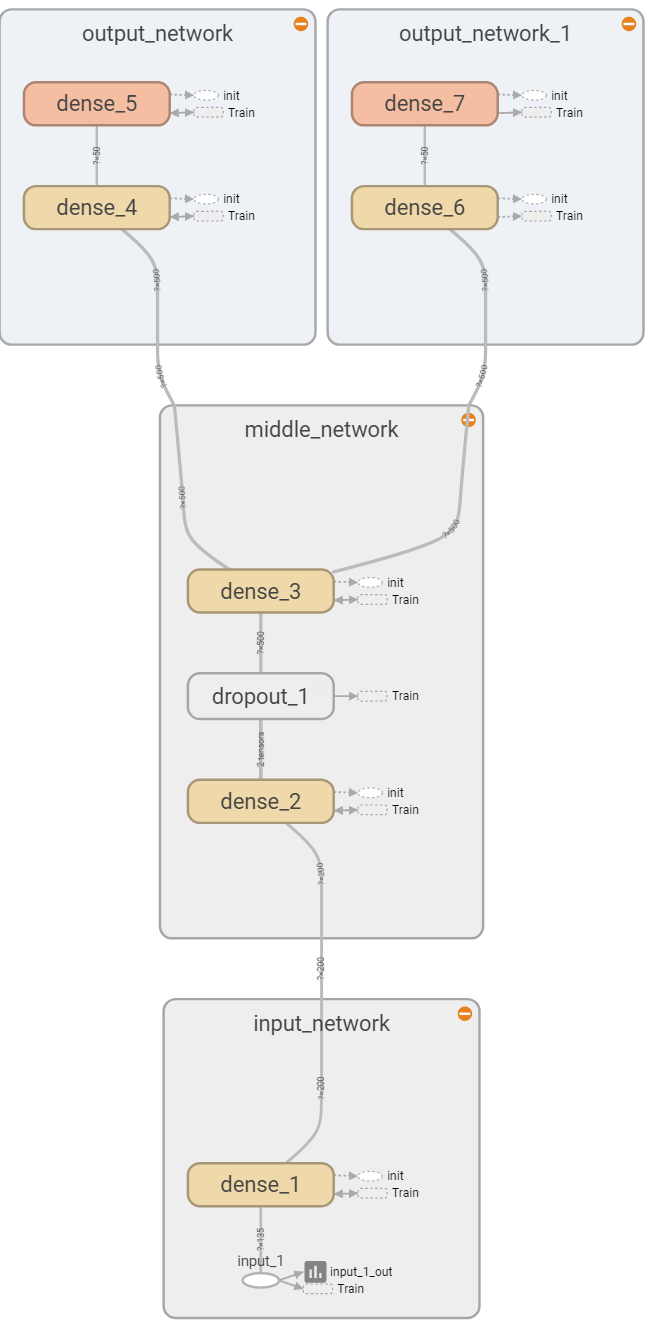
\includegraphics[scale=0.74]{Images/multiple_roles_expanded.png}
    \label{fig:multi_role_model}
\end{figure}



\begin{figure*}
    \caption{Muti-role model for Connect four}
    \begin{lstlisting}[language=Python, frame=single]
with tf.name_scope("input_network"):
in_con4 = Input(shape=(135,))
con4 = Dense(200, activation='relu')(in_con4)

with tf.name_scope("middle_network"):
mid = Dense(500, activation='relu')(con4)
mid = Dropout(0.5)(mid)
mid = Dense(500, activation='relu')(mid)

models = []
for i in range(2):
    with tf.name_scope("output_network"):
        out = Dense(50, activation='relu')(mid)
        out = Dense(8, activation='softmax')(out) 
        models.append(Model(inputs=in_con4, outputs=out))

# models = [role0, role1]
    \end{lstlisting}
    \label{fig:multi_role_model_code}
\end{figure*}
\begin{figure*}
    \centering
    \caption{Multi-gane model. This network is created with Kears. It has multiple inputs and multiple outputs, where each input is a game state and the outputs are the roles for those games. Image generated by Tensorboard. }
    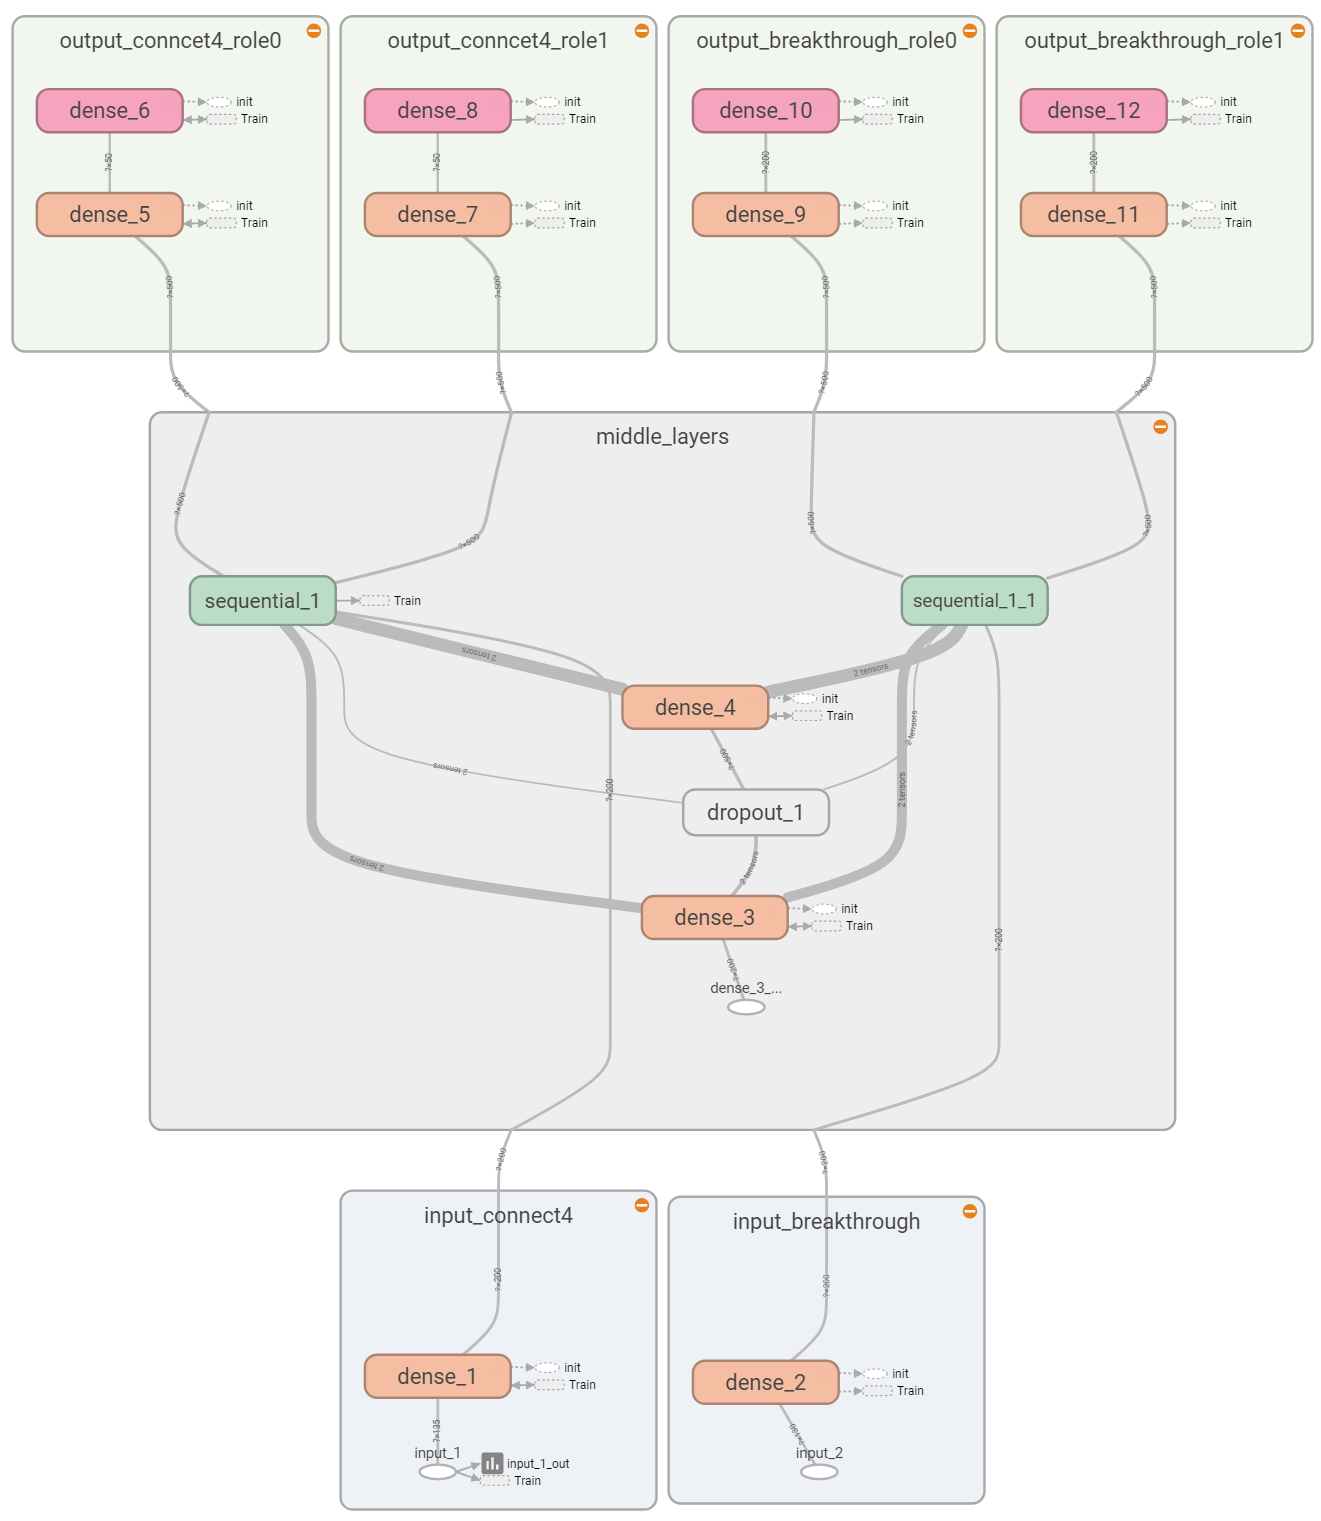
\includegraphics[scale=0.75]{Images/multiple_games_expanded.png}
    \label{fig:multi_game_model}
\end{figure*}

\end{document}


